\section{Zipper and one-holed contexts}

\section{Differentiation and contexts}

\subsection{Regular types}

\subsection{Container types}

\section{Generic zipper -- differentiating navigation}

In this section we build a bridge between Oleg Kiselyov's Haskell
implementation of the generic zipper. This is a transliteration of his
original code. As such, we provide a veneer over \texttt{Scala}'s
native delimited continuation library. Then we use this veneer to
express a direct translation of Oleg's code.

\begin{lstlisting}[language=Scala,mathescape=true]
  object MonadDefns {
    type MonadLike = { 
      def map[A,B]( f : A => B )
      def flatMap[M[_],A,B]( f : A => M[B] )
      def filter[A]( p : A => Boolean )    
    }
    type MonadXFormLike = {
      def lift[ML[_],MU[_],A]( m : ML[A] ) : MU[A]
    }
  }

  trait StateT[S,M[_],A]{
    def runState( s : S ) : M[(A,S)]
    def evalState( s : S ) : M[A]
    def get : StateT[S,M,S]
    def put( s : S ) : StateT[S,M,Unit]
    
    def map[B]( f : A => B )
    def flatMap[B]( f : A => StateT[S,M,B] )
    def filter( p : A => Boolean )
    
    def lift( c : M[A] ) : StateT[S,M,A]
  }

  trait CC[R,M[_],A] {
    def k2P : K[R,M,A,_] => StateT[Int,M,A]
  }

  trait Prompt[R,A] {
    def level : Int
  }

  class CPrompt[R,A](
    override val level : Int
  ) extends Prompt[R,A] {
  }

  trait P[R,M[_],A] {
    self : StateT[Int,M,A] =>
    def stateT : StateT[Int,M,A]
    def runP() : M[(Int,A)] 
    def newPrompt() = {
      for( n <- get ) yield{ put( n+1 ); new CPrompt( n ) }
    }
  }

  trait Frame[M[_],R,A,B]{
    def a2CC : A => CC[R,M,B]
  }

  trait K[R,M[_],A,B]{
    def frame : Frame[M,R,A,B]
    def r : R
    def a : A
    def b : B
    
    def map[C]( f : A => C )
    def flatMap[C]( f : A => K[R,M,A,C] )
    def filter( p : A => Boolean )
    
    def lift( m : M[A] ) : CC[R,M,A]
  }
  
  trait SubK[R,M[_],A,B] extends K[R,M,A,B]{
  }

  trait ControlOps[R,M[_],A] {
    def appk[B]( k : K[R,M,A,B], a : A ) : StateT[Int,M,A]
    def runCC( cc : CC[R,M,A] ) : M[A]
    def newPrompt( ) : CC[R,M,Prompt[R,A]]
    def pushPrompt(
      prompt : Prompt[R,A], cc : CC[R,M,A]
    ) : CC[R,M,A]
    def letSubK[B](
      prompt : Prompt[R,B],
      subk : SubK[R,M,A,B] => CC[R,M,B]
    ) : CC[R,M,A]
    def pushSubK[B](
      prompt : Prompt[R,B],
      subk : CC[R,M,A] 
    ) : CC[R,M,B]
    def promptP( f : Prompt[R,A] => CC[R,M,A] ) : CC[R,M,A]
    def shiftP[B](
      p : Prompt[R,B],
      f : (CC[R,M,A] => CC[R,M,B]) => CC[R,M,B]
    ) : CC[R,M,A]
}
\end{lstlisting}

Essentially, a zipper in this new style wraps a term. It may also
contain a traversal function.

\begin{lstlisting}[language=Scala,mathescape=true]  
  trait Zipper[R,M[_],T,D] {
    def term : T
  }

  class DCZipper[R,M[_],T,D](
    override val term : T,
    val traversal : CC[R,M,(Option[T],D)] => CC[R,M,Zipper[R,M,T,D]]
  ) extends Zipper[R,M,T,D]

  class ZipDone[R,M[_],T,D](
    override val term : T
  ) extends Zipper[R,M,T,D]
\end{lstlisting}

\break

We then provide basic factory mechanism for constructing zippers and
then using them.

\begin{lstlisting}[language=Scala,mathescape=true]
  trait ZipperOps[R,M[_],T,D] {
    def zipTerm(
      traversal
      : ( ( T => CC[R,M,( Option[T], D )] ), T )
        => CC[R,M,T],
      term : T
    ) : CC[R,M,Zipper[R,M,T,D]]
    def zipThrough( zipper : Zipper[R,M,T,D] ) : Unit
  }
\end{lstlisting}

\subsection{Delimited continuations}

In \texttt{Scala} we have the delimited continuations plugin. This
provides access to a type-driven source-to-source
continuation-passing-style translation of code involving the operators
\lstinline[language=Scala,mathescape=true]!shift! and
\lstinline[language=Scala,mathescape=true]!reset! to code that does
not. This approach has several interesting and novel features,
including a so-called ``direct-style'' syntax to express the
operations of delimited continuations.

This direct-style syntax is to be contrasted with a monadic
presentation of delimited continuations, as discovered by Dybvig,
Peyton-Jones and Sabry. One of the criticisms of this approach is that
it involves the use of a monadic ``meta-language''. That is, access to
the delimited continuations functionality requires using the monadic
operations plus some additional ones. However, assuming we have a
monad, \lstinline[language=Scala,mathescape=true]!T! supporting the
semantics for usual cast of
\lstinline[language=Scala,mathescape=true]!map!,
\lstinline[language=Scala,mathescape=true]!flatMap! and
\lstinline[language=Scala,mathescape=true]!filter!, together with four
additional operations --
\lstinline[language=Scala,mathescape=true]!newPrompt!,
\lstinline[language=Scala,mathescape=true]!pushPrompt!,
\lstinline[language=Scala,mathescape=true]!withSubCont! and
\lstinline[language=Scala,mathescape=true]!pushSubCont! -- we can use
\lstinline[language=Scala,mathescape=true]!for!  comprehensions
together with the prompt and sub-continuation operations as a DSL for
delimited continuations. We only need source-to-source translations
for embedded use of the prompt and subcontinuation operations -- i.e.,
occurrences of the those operations inside a
\lstinline[language=Scala,mathescape=true]!for! comprehension -- which
we give below.

\break

\begin{lstlisting}[language=Scala,mathescape=true]    
  $\mathcal{T}\ldb$ newPrompt $\rdb$ = newPrompt
  $\mathcal{T}\ldb$ pushPrompt $e_{1} \; e_{2}$ $\rdb$ =
     $\mathcal{T}\meaningof{e_1}$ flatMap {
       ( p ) => pushPrompt p $\mathcal{T}\meaningof{e_2}$
     }
  $\mathcal{T}\ldb$ withSubCont $e_1 \; e_2$ $\rdb$ =
     $\mathcal{T}\meaningof{e_1}$ flatMap {
       ( p ) => $\mathcal{T}\meaningof{e_2}$ flatMap {
         ( f ) => withSubCont p f
       }
     }
  $\mathcal{T}\ldb$ pushSubCont $e_1 \; e_2$ $\rdb$ =
     $\mathcal{T}\meaningof{e_1}$ flatMap {
       ( s ) => pushSubCont s $\mathcal{T}\meaningof{e_2}$
     }
\end{lstlisting}

This would allow an alternative presentation of delimited
continuations which has the advantage of facilitating
``transliteration'' of \texttt{Haskell} packages dependent on the
widely used Dybvig-Peyton-Jones-Sabry approach.

\subsubsection{The genericity of delimited continuations}

In previous sections we have used the analogy of monads as maintaining
a discipline for "putting things in a box"; similarly, comonads
provide a discipline for "taking things out of the box". There is a
connection between this and delimited continuations. To see the
connection, we might imagine a picture like

\begin{figure}[tbp]
\begin{center}
{ 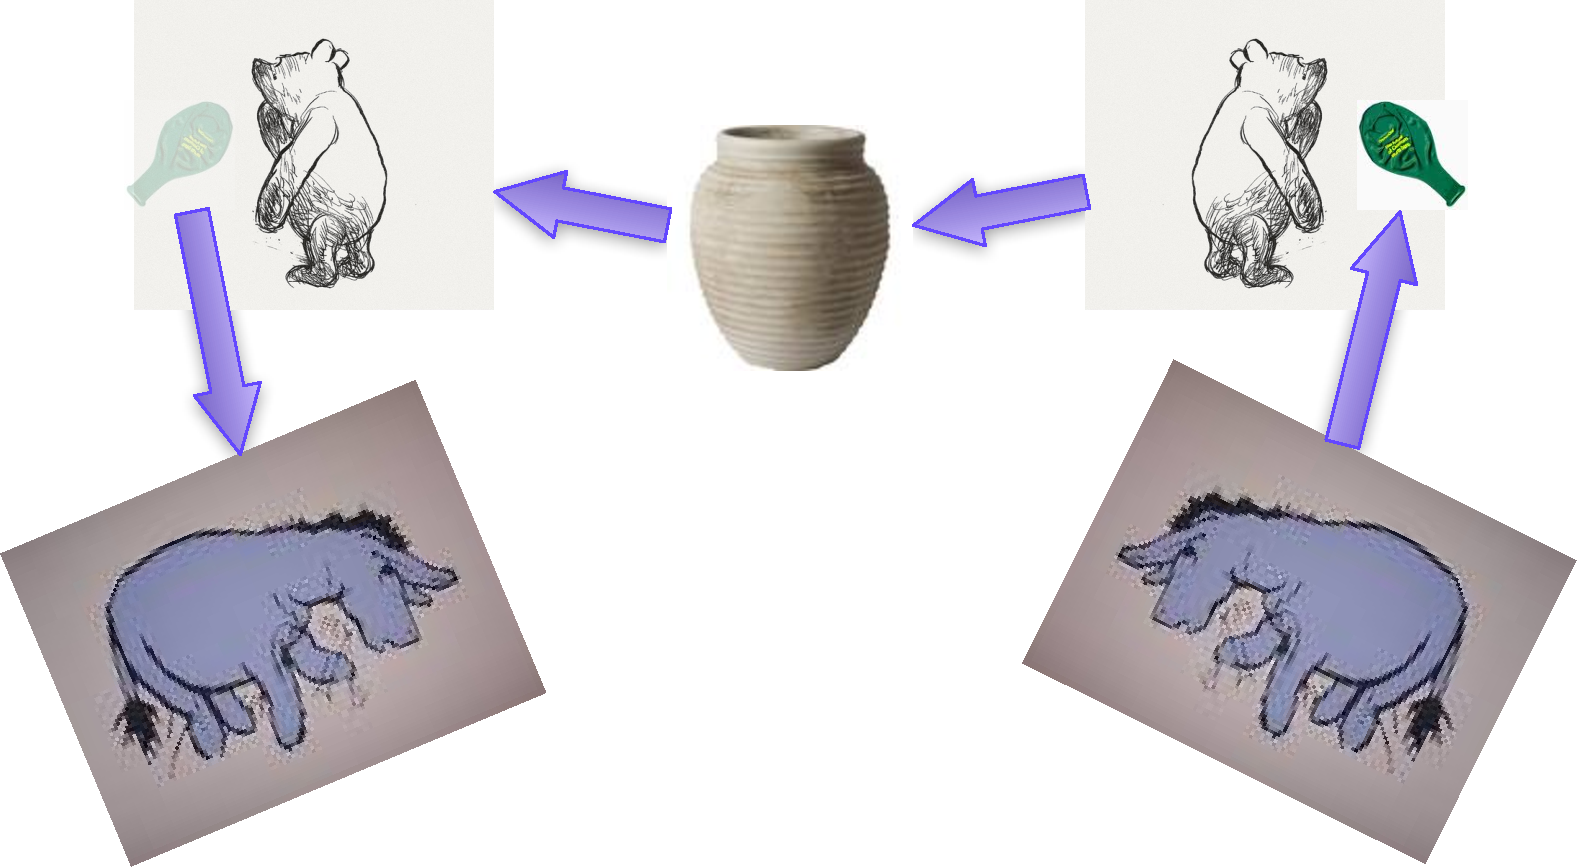
\includegraphics[scale=.35]{/Users/lgm/work/src/projex/biosimilarity/trace/src/main/book/content/figures/ProducerConsumerEeyoreNPoohInitial.pdf} }
\caption{ delimited continuations and synchronized exchange  }
\end{center}
\end{figure}

One way to implement this is that the ``daemon'', Pooh, is really just
the act of wrapping either client's access to the box in code that
grabs the current continuation, call it kg (or kt, respectively), and
then does the following.  
\begin{itemize}
  \item Giver side: 
    \begin{figure}[tbp]
      \begin{center}
        { 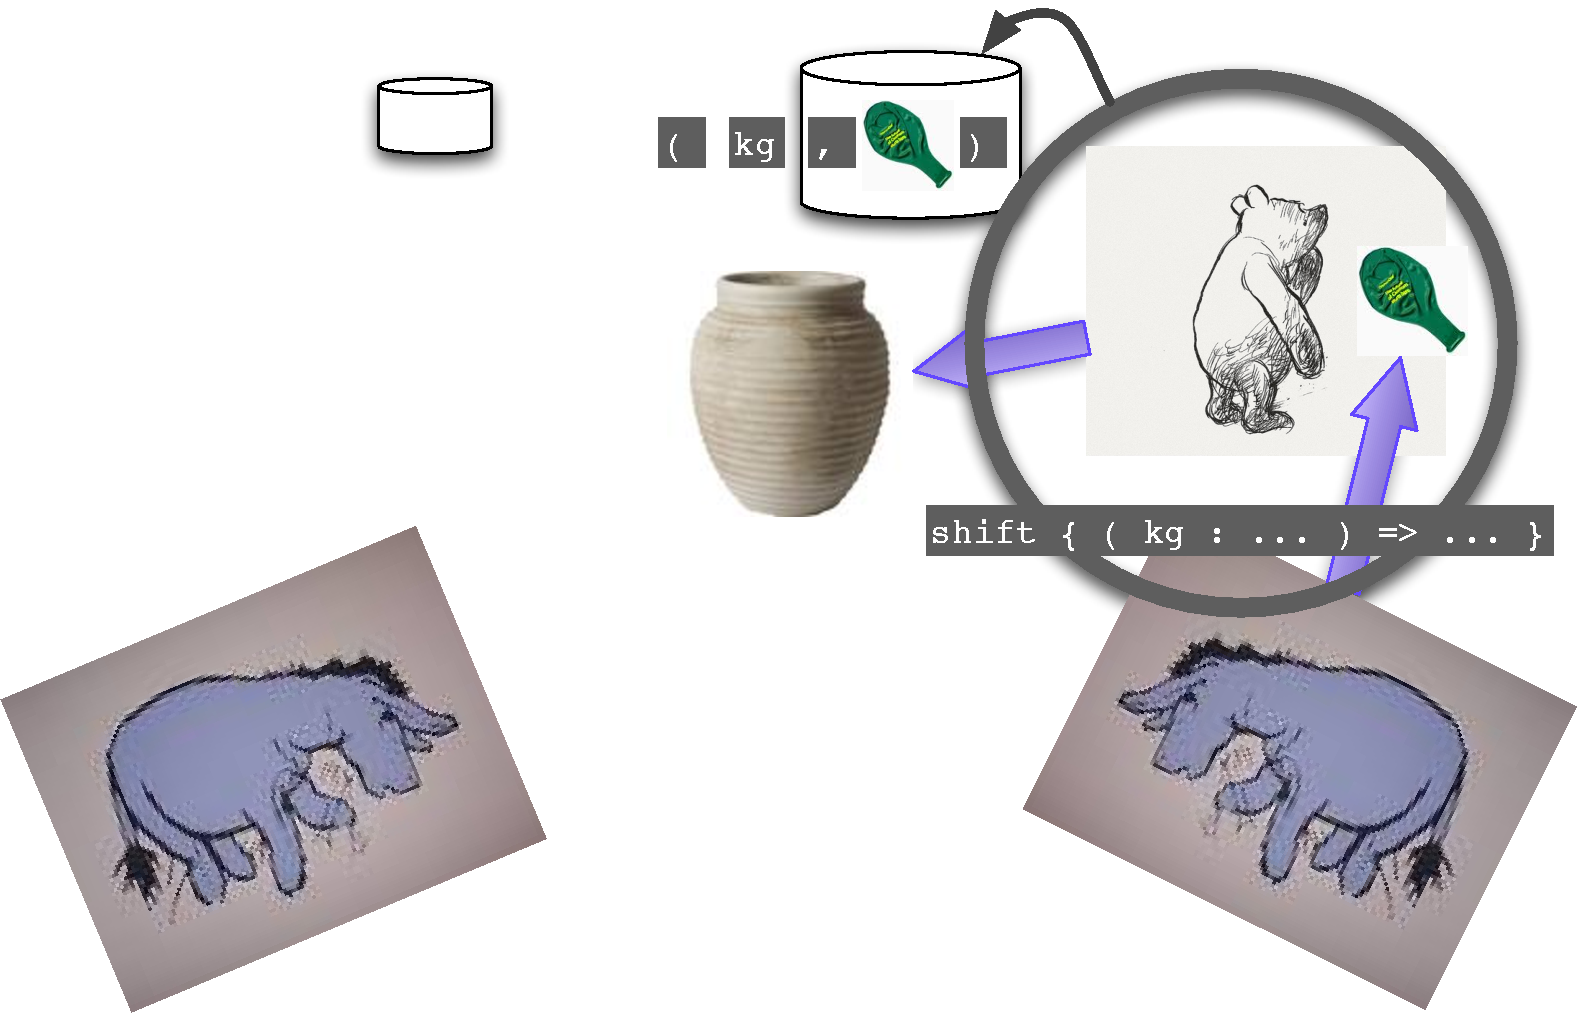
\includegraphics[scale=.35]{/Users/lgm/work/src/projex/biosimilarity/trace/src/main/book/content/figures/ProducerConsumerEeyoreNPoohSupply.pdf} }
        \caption{ Giver's side }
      \end{center}
    \end{figure}
    \begin{itemize} 
    \item check to see if there is a matching taker, kt, (in a queue
      of taker requests packaged as continuations). 
    \item If there is, invoke (kt v) passing it the value, v, that
      came in on the giver's call, and invoke (kg unit), passing it
      unit. 
    \item Otherwise, queue (v,kg) in a giver's queue.
    \end{itemize}
  \item Taker's side:
    \begin{figure}[tbp]
      \begin{center}
        { 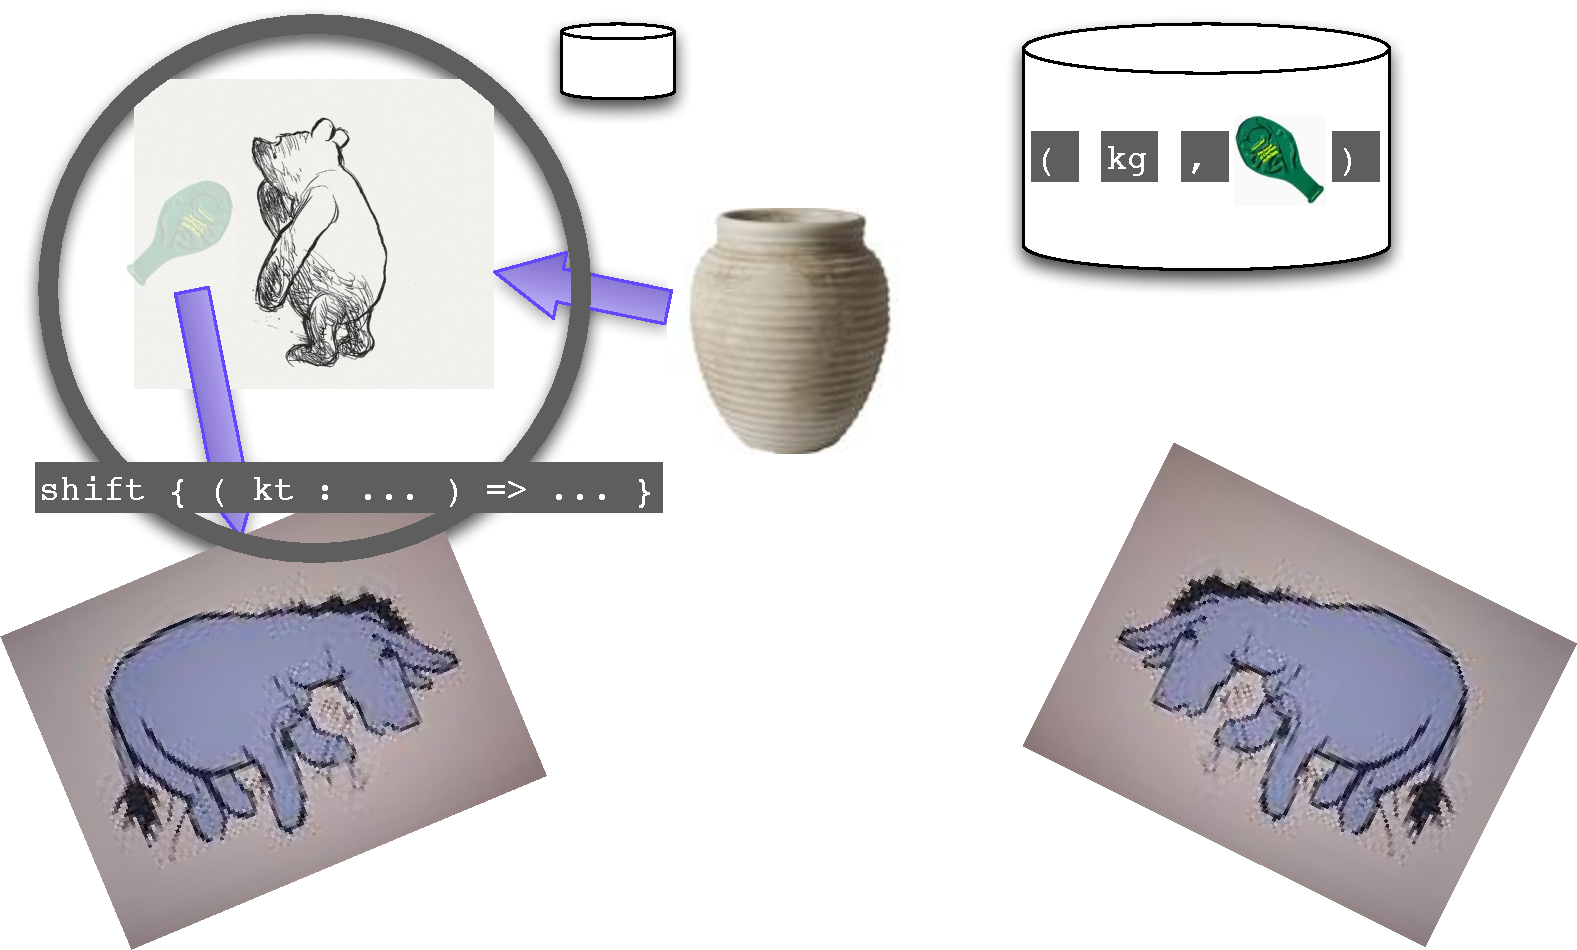
\includegraphics[scale=.35]{/Users/lgm/work/src/projex/biosimilarity/trace/src/main/book/content/figures/ProducerConsumerEeyoreNPoohRequest.pdf} }
        \caption{ Taker's side }
      \end{center}
    \end{figure}
    \begin{itemize}
    \item check to see if there is a matching giver, (v,kg),
      (in a queue of giver requests packages as continuations).
    \item If there is, invoke (kt v), passing v to the taker's
      continuation, and (kg unit) passing unit to the giver's
      continuation.
    \item Otherwise, queue kt in a taker's queue.
  \end{itemize}
\end{itemize}

If these look strangely like the put and get operations of the State
monad -- they's because they are. They've been coordinated around a
state cell that is "located" at a rendezvous point for a pair of
coroutines to exchange data.

For the adventurous, it is possible to develop a further connection to
Milner's $\pi$-calculus. Roughly speaking, this is the way to
implement synchronous-IO-style in the $\pi$-calculus, spelling out a
specific relationship between delimited continuations and
$\pi$-calculus-style communication.

If you see a further connection between this pattern and tuple spaces,
that's because it's the basic mechanism for implementing tuple spaces.

Summarizing, monads like IO that are forever sticky, are one-way
monads. Like the roach motel, or Hotel California, things go in, but
don't come out. Monads that are really containers are
"intuitionistic". That is, you know that if you put something in, you
can get it out; but, if you receive a container, you don't know if it
has anything in it until you open the lid. They have a relationship
with a comonad that is "intuitionistically" disciplined. Finally,
there are monad-comonad pairs that enjoy a linear discipline. This
linear discipline matches every "gozinta" with a "gozouta" and vice
versa. That discipline may be implemented by delimited
continuations. This implementation strategy, by the way, also connects
delimited continuations to the other generic zipper, discovered by
Oleg.

\section{Species of Structure}